% !TeX program = pdflatex
\documentclass[border=6pt]{standalone}
\usepackage{amssymb}
\usepackage{tikz}
\usetikzlibrary{arrows.meta, positioning, calc}

\definecolor{MediumRed}{rgb}{0.925, 0.345, 0.345}
\definecolor{MediumGreen}{rgb}{0.37, 0.7, 0.66}
\definecolor{MediumBlue}{rgb}{0.015, 0.315, 0.45}
\definecolor{DarkBlue}{rgb}{0.05, 0.15, 0.35}

% figura de palo simple centrada en (0,0), escala ~1
\newcommand{\stick}[2]{% #1 = color cuerpo, #2 = color brazos
  \fill[#1] (0,0.55) circle (0.13);
  \draw[#1, line width=1.4pt] (0,0.42)--(0,-0.35);
  \draw[#2, line width=1.4pt] (-0.4,0.1)--(0,0.25)--(0.4,0.1);
  \draw[#1, line width=1.4pt] (0,-0.35)--(-0.28,-0.75);
  \draw[#1, line width=1.4pt] (0,-0.35)--(0.28,-0.75);
}

\begin{document}
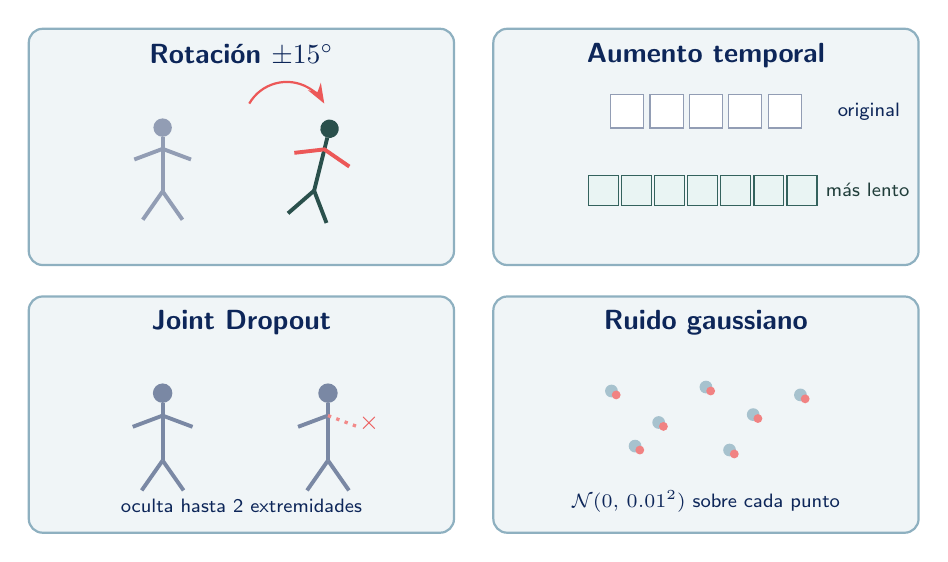
\begin{tikzpicture}[
    font=\sffamily,
    panel/.style={draw=MediumBlue!45, thick, rounded corners=5pt, fill=MediumBlue!6,
        minimum width=5.4cm, minimum height=3.0cm},
    tit/.style={font=\sffamily\bfseries, text=DarkBlue},
]

% ===== marco de los 4 paneles =====
\node[panel] (p1) at (0,0) {};
\node[panel] (p2) at (5.9,0) {};
\node[panel] (p3) at (0,-3.4) {};
\node[panel] (p4) at (5.9,-3.4) {};

% ===== 1: Rotacion =====
\node[tit] at ($(p1.north)+(0,-0.35)$) {Rotación $\pm 15^\circ$};
\begin{scope}[shift={($(p1.center)+(-1.0,-0.25)$)}, scale=0.9]
    \stick{DarkBlue!45}{DarkBlue!45}
\end{scope}
\begin{scope}[shift={($(p1.center)+(1.0,-0.25)$)}, rotate=-14, scale=0.9]
    \stick{MediumGreen!45!black}{MediumRed}
\end{scope}
\draw[-{Stealth[length=2.5mm]}, MediumRed, thick] ($(p1.center)+(0.1,0.55)$) arc (150:30:0.55);

% ===== 2: Aumento temporal =====
\node[tit] at ($(p2.north)+(0,-0.35)$) {Aumento temporal};
\foreach \i in {0,...,4}
    \node[draw=DarkBlue!45, fill=white, minimum size=0.42cm, inner sep=0]
        at ($(p2.center)+(\i*0.5-1.0,0.45)$) {};
% mas lento: duplica
\foreach \i in {0,...,6}
    \node[draw=MediumGreen!55!black, fill=MediumGreen!14, minimum size=0.38cm, inner sep=0]
        at ($(p2.center)+(\i*0.42-1.3,-0.55)$) {};
\node[font=\sffamily\scriptsize, text=DarkBlue, anchor=west] at ($(p2.center)+(1.55,0.45)$) {original};
\node[font=\sffamily\scriptsize, text=MediumGreen!35!black, anchor=west] at ($(p2.center)+(1.40,-0.55)$) {más lento};

% ===== 3: Joint Dropout =====
\node[tit] at ($(p3.north)+(0,-0.35)$) {\textit{Joint Dropout}};
\begin{scope}[shift={($(p3.center)+(-1.0,-0.25)$)}, scale=0.95]
    \stick{DarkBlue!55}{DarkBlue!55}
\end{scope}
\begin{scope}[shift={($(p3.center)+(1.1,-0.25)$)}, scale=0.95]
    % cuerpo visible, brazo derecho ocluido (rojo punteado)
    \fill[DarkBlue!55] (0,0.55) circle (0.13);
    \draw[DarkBlue!55, line width=1.4pt] (0,0.42)--(0,-0.35);
    \draw[DarkBlue!55, line width=1.4pt] (-0.4,0.1)--(0,0.25);
    \draw[MediumRed!70, line width=1.2pt, dotted] (0,0.25)--(0.4,0.1);
    \draw[DarkBlue!55, line width=1.4pt] (0,-0.35)--(-0.28,-0.75);
    \draw[DarkBlue!55, line width=1.4pt] (0,-0.35)--(0.28,-0.75);
    \node[text=MediumRed, font=\small\bfseries] at (0.55,0.15) {$\times$};
\end{scope}
\node[font=\sffamily\scriptsize, text=DarkBlue, anchor=south] at ($(p3.south)+(0,0.15)$)
    {oculta hasta 2 extremidades};

% ===== 4: Ruido gaussiano =====
\node[tit] at ($(p4.north)+(0,-0.35)$) {Ruido gaussiano};
\foreach \x/\y in {-1.2/0.3,-0.6/-0.1,0/0.35,0.6/0.0,1.2/0.25,-0.9/-0.4,0.3/-0.45}{
    \fill[MediumBlue!35] ($(p4.center)+(\x,\y)$) circle (2.3pt);
    \fill[MediumRed!75] ($(p4.center)+(\x+0.06,\y-0.05)$) circle (1.6pt);
}
\node[font=\sffamily\scriptsize, text=DarkBlue, anchor=south] at ($(p4.south)+(0,0.15)$)
    {$\mathcal{N}(0,\,0.01^2)$ sobre cada punto};

\end{tikzpicture}
\end{document}
